\section{Deployment dei microservizi con Docker}

\subsection{Healthcheck}
L’healthcheck è una funzionalità di Docker che permette di definire dei controlli di salute sul container: specificando un comando da mandare in azione periodicamente, Docker controlla se il container è "vivo e in salute". Per capire se l'applicazione è sia "viva"(quindi online) che "in salute"(e quindi operativa), risulta cruciale la scelta del comando da mandare periodicamente in azione.

Alcuni applicativi, come il DBMS MariaDB adottato, contengono degli script dediti al controllo della salute del sistema (nel caso di MariaDB, essa contiene nel suo filesystem \textit{healthcheck.sh}, dedita proprio a questa operazione), mentre altri utilizzano delle operazioni note.

I microservizi in Spring Boot, in particolare, hanno la possibilità di installare la dipendenza \textit{Actuator}\cite{halthcheck} che consente l'healthcheck. Tale dipendenza espone una API apposita per restituire lo stato in salute dell'applicativo. E' stato possibile quindi utilizzare l'API \texttt{/actuator/health} del microservizio per effettuare un controllo periodico del suo stato in salute. 

L'healthcheck può inoltre servire per valutare la salute complessiva della rete di microservizi: è possibile introdurre un vincolo di dipendenza tra i componenti di sistema affinchè un certo container vada online solo se i container da cui è dipendente sono "vivi e in salute".

\subsection{Setup della rete di microservizi}
Viene impostato il \textit{docker-compose.yaml} esplicitando i microservizi che compongono l'architettura. Spring Boot dà la possibilità di impostare le variabili ambientali sui container Docker Compose, in modo da sovrascrivere le proprietà definite nel \textit{application.yaml} e \textit{application.properties}. 
In questo modo, è possibile riadattare l'esecuzione dei microservizi per assumere un'impostazione su misura per la runtime in rete.

\begin{lstlisting}[language=docker-compose,caption={GestioneCucina con healthcheck, dipendenze e variabili sovrascritte},label=lst:healthcheck]
|@\color{codeMediumDarkblue}\textbf{GestioneCucina}|@:
    image: gchirico1/gestione_cucina:latest
    container_name: GestioneCucina
    restart: always
    environment:
      |@\color{codeMediumDarkblue}\textbf{SERVER\_PORT}|@: 8080
      |@\color{codeMediumDarkblue}\textbf{SERVER\_ADDRESS}|@: 0.0.0.0
      |@\color{codeMediumDarkblue}\textbf{SPRING\_DATASOURCE\_URL}|@: jdbc:mariadb://db:3306/serveeasy
      |@\color{codeMediumDarkblue}\textbf{SPRING\_KAFKA\_BOOTSTRAP-SERVERS}|@: broker:29092 #plaintext_internal
    depends_on:
      |@\color{codeMediumDarkblue}\textbf{broker}|@:
        |@\color{codeMediumDarkblue}\textbf{condition}|@: service_healthy
      |@\color{codeMediumDarkblue}\textbf{db}|@:
        |@\color{codeMediumDarkblue}\textbf{condition}|@: service_healthy
    |@\color{codeMediumDarkblue}\textbf{healthcheck}|@:
        |@\color{codeMediumDarkblue}\textbf{test}|@: "curl --fail --silent localhost:8080/actuator/health | grep UP || exit 1"
        |@\color{codeMediumDarkblue}\textbf{interval}|@: 20s
        |@\color{codeMediumDarkblue}\textbf{timeout}|@: 5s
        |@\color{codeMediumDarkblue}\textbf{start\_period}|@: 40s
    |@\color{codeMediumDarkblue}\textbf{expose}|@:
      - "8080"
    ports:
      - "8082:8080"
\end{lstlisting}

\subsection{Attivazione della rete di microservizi}
Oltre al comando \texttt{docker compose up}, è possibile attivare e gestire la rete da Intellij IDEA. Quest'ultima modalità è risultata molto più comoda per il controllo della salute e delle attività della rete: il cruscotto offerto dall'IDE consente, infatti, una visuale completa e dettagliata di ogni log in tempo reale. 

Attivato il \textit{docker-compose.yml}, vengono scaricati i microservizi da Dockerhub e attivati i container seguendo la sequenza specificata attraverso le dipendenze.

\begin{figure}[htbp]
	\centering
	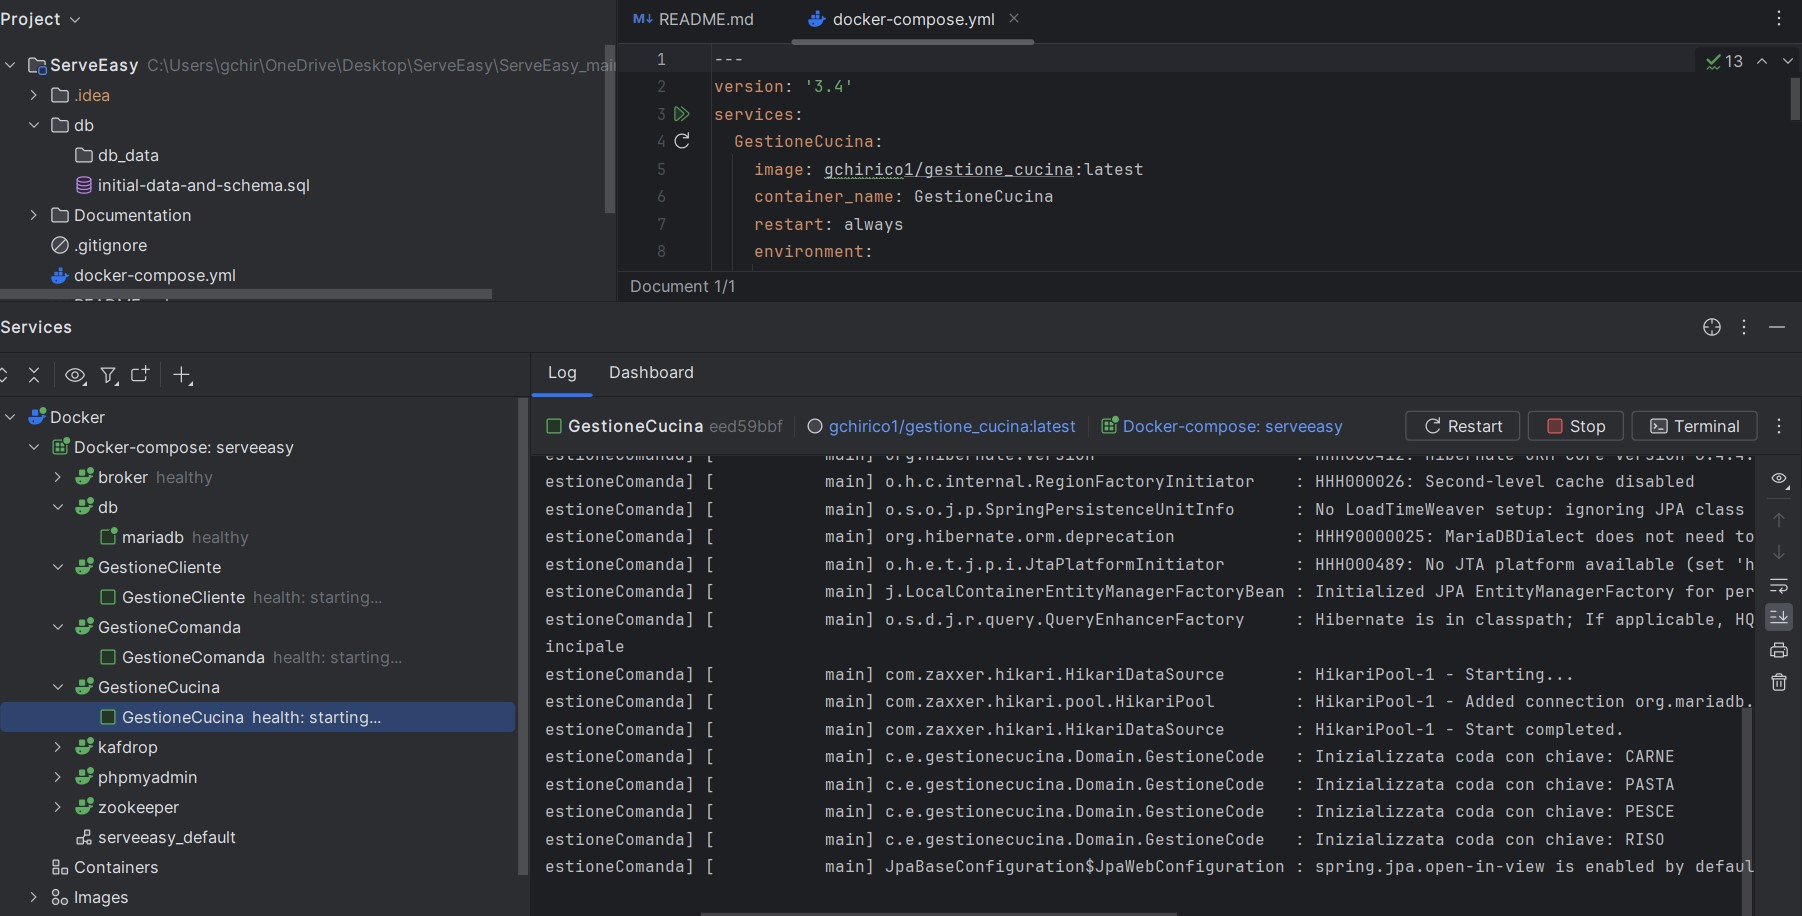
\includegraphics[scale=0.40]{iterazione1/images/startup.jpg}
	\caption{Startup della rete, inizializzazione code in GestioneCucina
 \label{fig:startupcucina}}
\end{figure}
\clearpage